Flavour-changing neutral currents (FCNC) have played a significant role
in the construction of the Standard Model of particle physics (SM).
These processes are forbidden at tree level and can proceed only via loops,
hence are rare. An important set of FCNC processes involve the transition
of a b quark to an s quark and two leptons, process mediated by
electroweak box and penguin diagrams as shown in Fig.~\ref{intro:fig:diagrams}.
If heavy new particles exist, they may contribute to FCNC decay amplitudes,
affecting the measurement of observables related to the decay under study.
Hence FCNC processes allow searches for contributions from sources of physics
beyond the SM (hereafter referred to as new physics).
These decays can also be exploited to test Lepton Flavour Universality
(LFU): in the SM the electroweak gauge bosons $Z$ and $W^{\pm}$ have
identical couplings to all three lepton flavours. Hence the branching
fractions of decays involving different lepton families do not depend
on the lepton flavour, but only on phase space and helicity considerations.
Any experimental evidence of violation of LFU would be a clear sign
of physics beyond the SM (BSM).

\begin{figure}[h]
\begin{center}
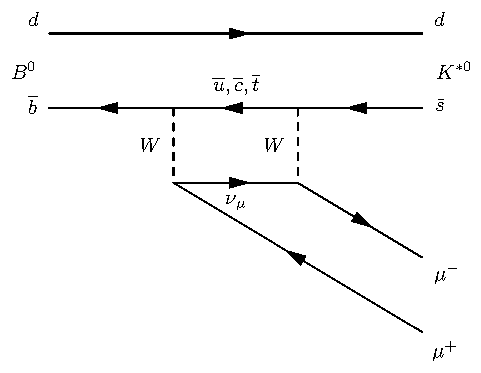
\includegraphics[width=0.45\textwidth]{figures/Feynman_diagrams-box.pdf}
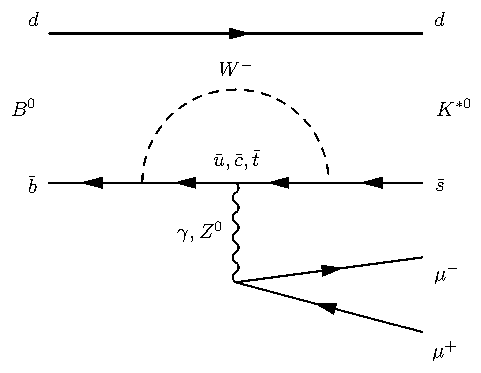
\includegraphics[width=0.45\textwidth]{figures/Feynman_diagrams-penguin.pdf}
\caption{Box and penguin Feynman diagrams of \bkstmumu decay.}
\label{intro:fig:diagrams}
\end{center}
\end{figure}

In the SM, the ratio of branching fractions of these decays is predicted to
be about unity, as the electron and muon masses are very small with respect
to that of the $b$ quark. The ratio can deviate from unity, when the value
of the dilepton invariant mass-squared ($q^2$) increases,
reducing the phase space available to the two final-state leptons.
Hence, in general the ratio is defined over a $q^2$ range $[q^2_{\mathrm min}, q^{2}_{\mathrm max}]$ as

\begin{equation}
  \label{intro:eq:rq2}
  R_{\mathrm{LFU}} \equiv \dfrac{\displaystyle\int_{q^2_{\mathrm min}}^{q^2_{\mathrm max}}
  \dfrac{\mathrm{d}\BR(\bhmumu)}{\mathrm{d}\qsqr} \mathrm{d}\qsqr}
  {\displaystyle\int_{q^2_{\mathrm min}}^{q^2_{\mathrm max}} \dfrac{\mathrm{d}\BR(\bhee)}{\mathrm{d}\qsqr} \mathrm{d}\qsqr} ~.
\end{equation}

From the experimental point of view, the detection and measurement of the
two channels with the two lepton types exploit different parts of the detector,
different reconstruction techniques and different efficiencies.
Hence a double ratio can be defined where the decays of interest are compared
with the corresponding resonant decays used as reference channels:

\begin{equation}
  \label{intro:eq:doubleratio}
  \rkst = {\frac{\BR(\bkstmumu)}{\BR(\bkstjpsimumu)}} \bigg{/} {\frac{\BR(\bkstee)}{\BR(\bkstjpsiee)}} \, .
\end{equation}


%Hereafter, the K*(892)is referred to asK∗and charge conjugation is implied
%throughout, unless stated otherwise. ratio of rates of decay into dimuon and
%dielectron final states,all as a function of the invariant mass squared
%of the dilepton systemq2. All of these observable sets canbe sensitive
%to different types of new physics that allow for FCNCs
%at tree or loop level. The BaBar, Belle,CDF, CMS, and LHCb collaborations
%have published the results of studies of the angular distributions for
%B0d→K∗μ+μ−[1–8]. The LHCb Collaboration has reported a potential hint,
%at the level of3.4standarddeviations, of a deviation from SM calculations
%[3, 4] in this decay mode when using a parameterizationof the angular
%distribution designed to minimise uncertainties from hadronic form
%factors. Measurementsusing this approach were also reported by the
%Belle and CMS Collaborations [6, 8] and they are consistentwith the
%LHCb experiment’s results and with the SM calculations. This paper
%presents results followingthe methodology outlined in Ref. [3] and
%the convention adopted by the LHCb Collaboration for thedefinition
%of angular observables described in Ref. [9].
